
We present simulation results that illustrate the core mechanism driving misinformation diffusion and examine how platform-level fact-checking policies impact spread dynamics. Our analysis focuses on understanding how reputation-based filtering operates in heterogeneous networks and how varying fact-checking capabilities across platforms (comparing WhatsApp's higher fact-checking rates to Telegram's lower rates) affects contamination patterns.

\subsection{The Reputation-Based Filtering Mechanism}

The central mechanism in our model operates through a reputation feedback loop: agents with higher reputation have much more to lose from forwarding false messages (via $\delta(\R) = \delta_0 \cdot \sigma(\R) \cdot (1 + \sigma(\R))$), while the gain from forwarding true messages is constant (via $\gamma = \gamma_0$). Because $\delta(\R)$ rises steeply with reputation (up to $2\delta_0$), high-reputation agents become increasingly selective over time.

When agents form beliefs about message truthfulness, they rely on two signals: (i) ideological proximity $\phi(\bias_i, \bias_m)$ and (ii) sender reputation $\sigma(\R_j)$. Agents forward messages when expected utility $\mathbb{E}[u] = \omega \phi + \gamma \belief - \delta(\R)(1-\belief) - \cost \geq 0$. As $\delta(\R)$ is larger for high-reputation agents, they require stronger signals (higher $\belief$) to forward, making them natural filters.

Figure~\ref{fig:reputation_step3} illustrates this mechanism: influencers (high initial reputation) maintain elevated reputation levels through selective forwarding, while bots (low reputation sensitivity) show stable low reputation. Regular users, with moderate reputation parameters, exhibit intermediate behavior. This reputation divergence reinforces behavioral differences over time, creating a self-reinforcing filtering system.

\begin{figure}[H]
\centering
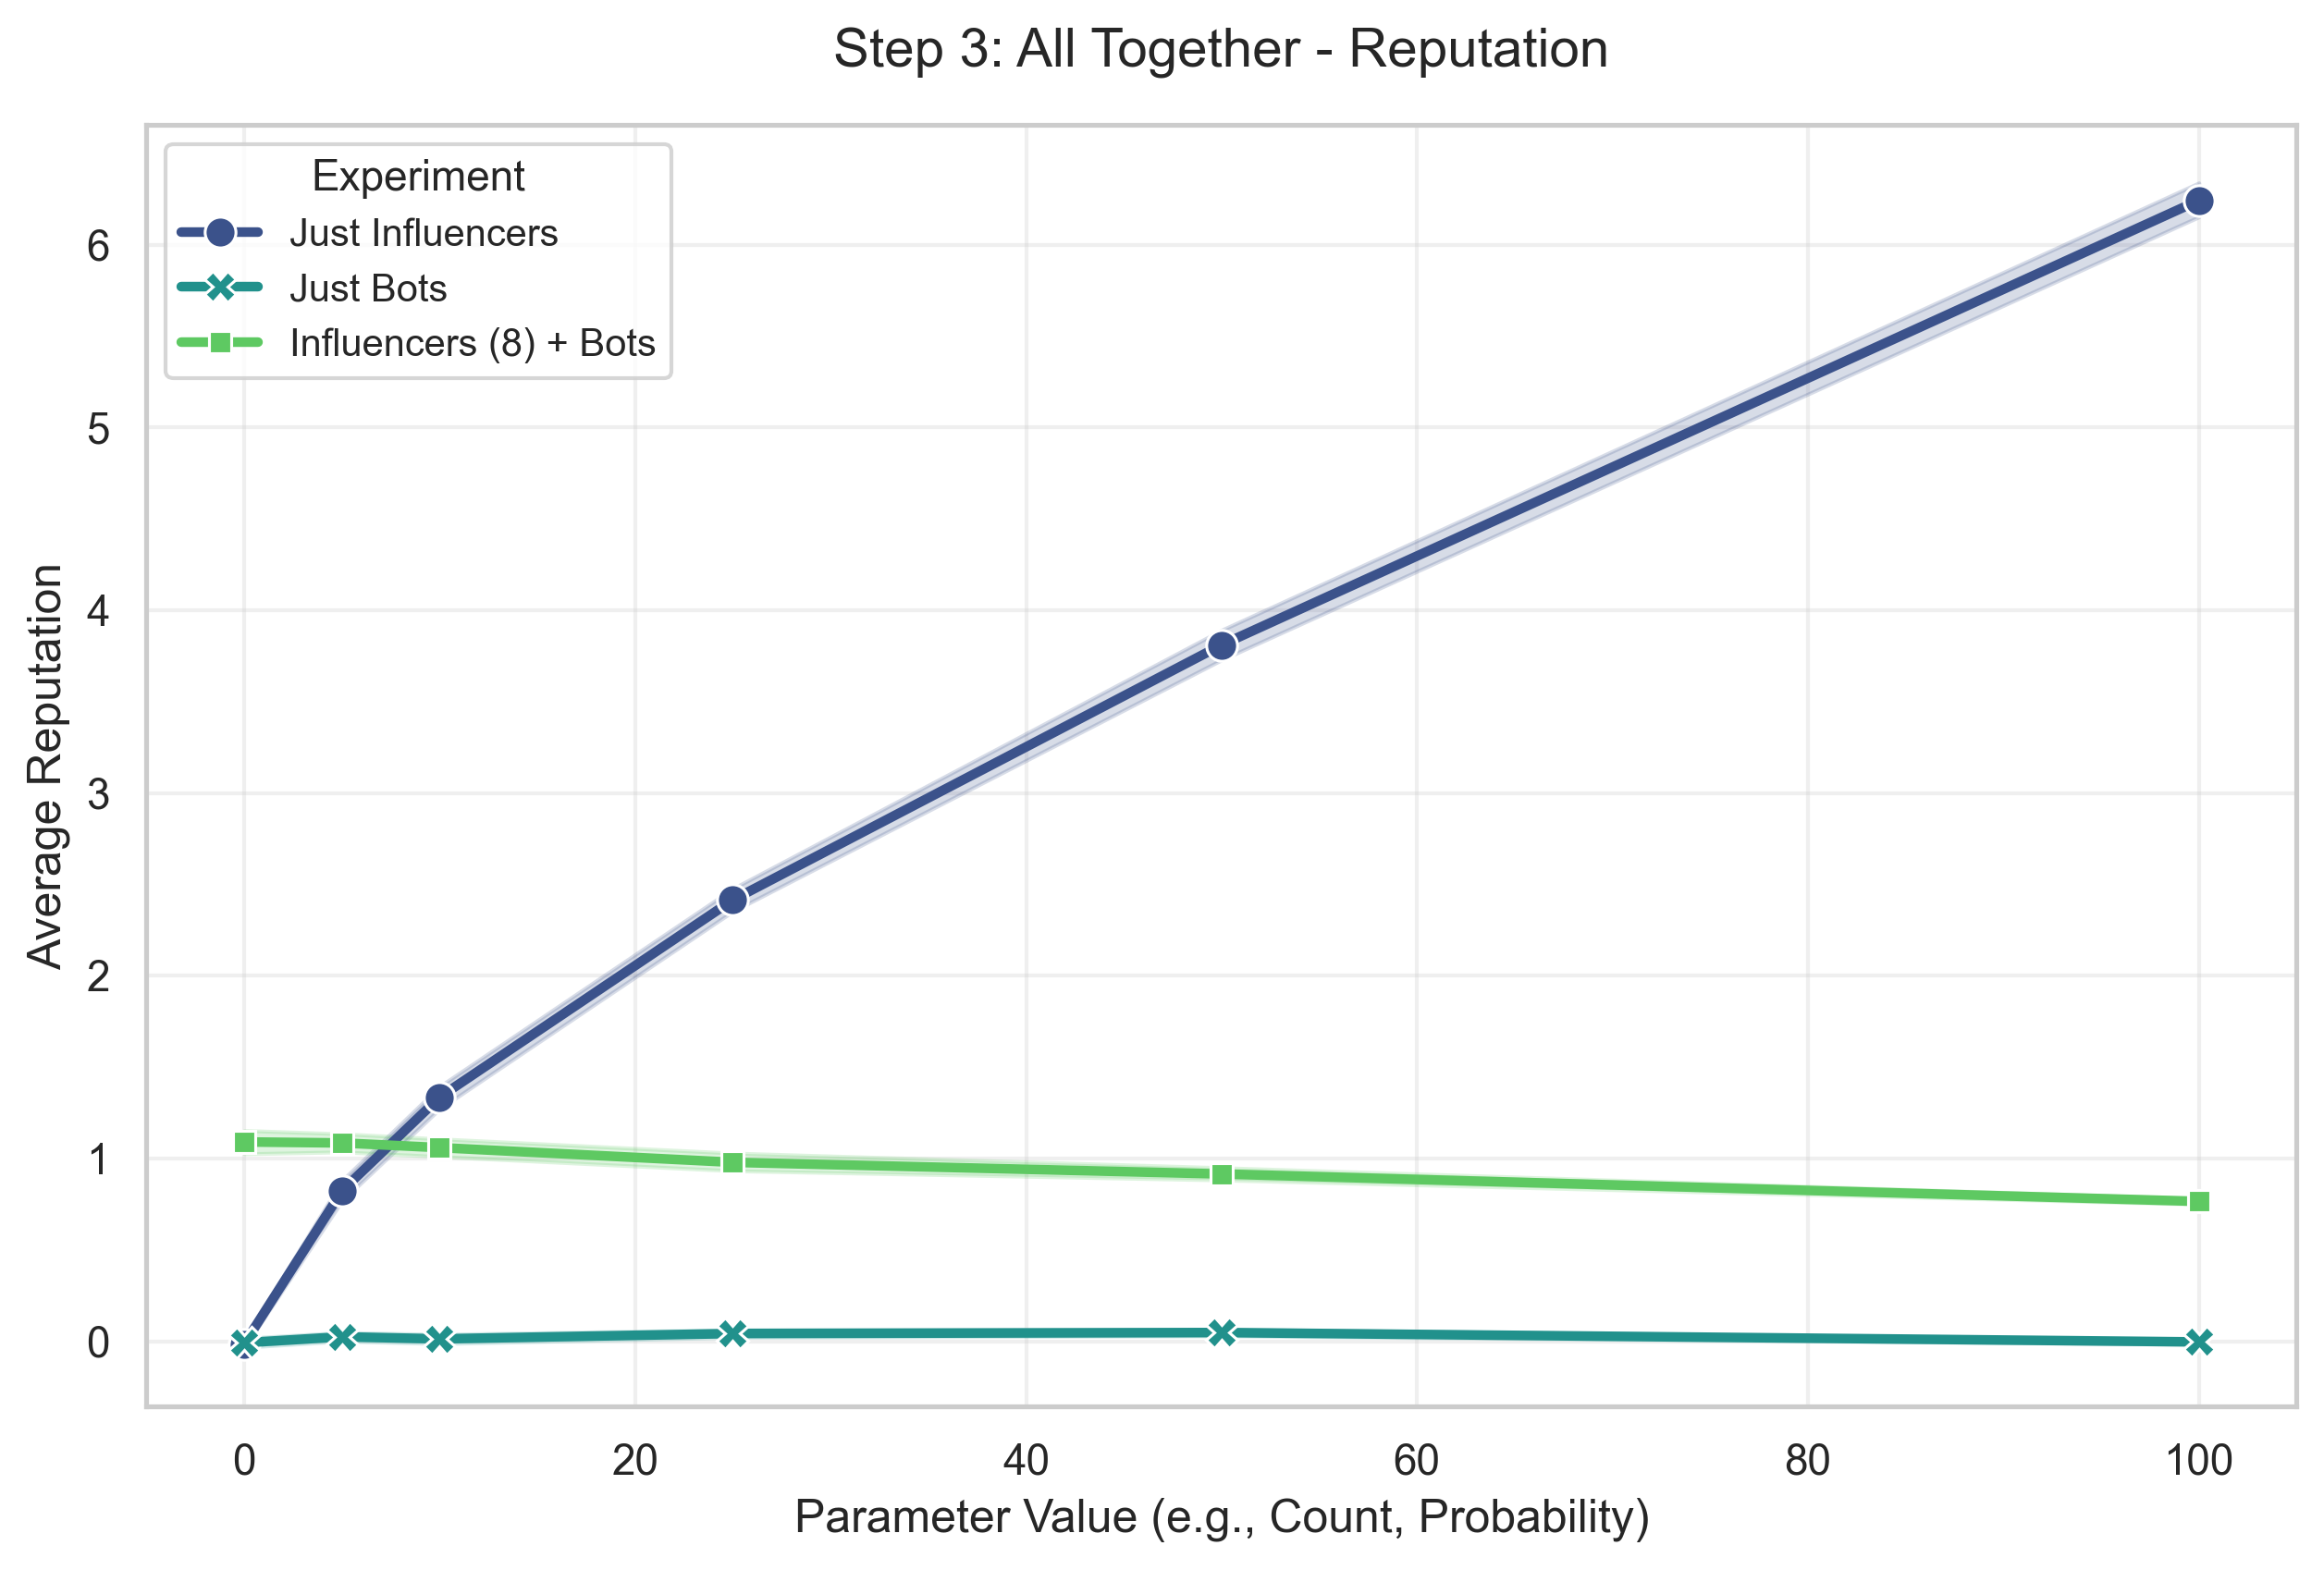
\includegraphics[width=0.8\textwidth]{figures/reputation_step3_all.png}
\caption{Reputation evolution showing the filtering mechanism: high-reputation agents maintain credibility through selective forwarding, while low-reputation agents show stable low values.}
\label{fig:reputation_step3}
\end{figure}

\subsection{Key Findings on Diffusion Patterns}

Our simulations reveal several important patterns in how this mechanism shapes misinformation spread:

\begin{enumerate}
    \item \textbf{Reputation as endogenous filter}: The penalty $\delta(\R) = \delta_0 \cdot \sigma(\R) \cdot (1 + \sigma(\R))$ is much larger for high-reputation agents, creating a feedback loop that makes them increasingly selective. This aggressive filtering significantly reduces misinformation contamination among high-reputation agents, as they require much stronger signals before forwarding.
    
    \item \textbf{Heterogeneous agent roles}: Influencers act as natural filters but can be bypassed by bots and regular users. Regular users serve as bridges between clusters, facilitating cross-community spillovers that enable misinformation to escape local containment.
    
    \item \textbf{Network amplification}: Even when reputation-sensitive agents filter effectively at the individual level, network structure can amplify spread. The presence of low-reputation agents (bots) significantly increases contamination rates, as shown in Figure~\ref{fig:misinformation_step3}.
\end{enumerate}

\begin{figure}[H]
\centering
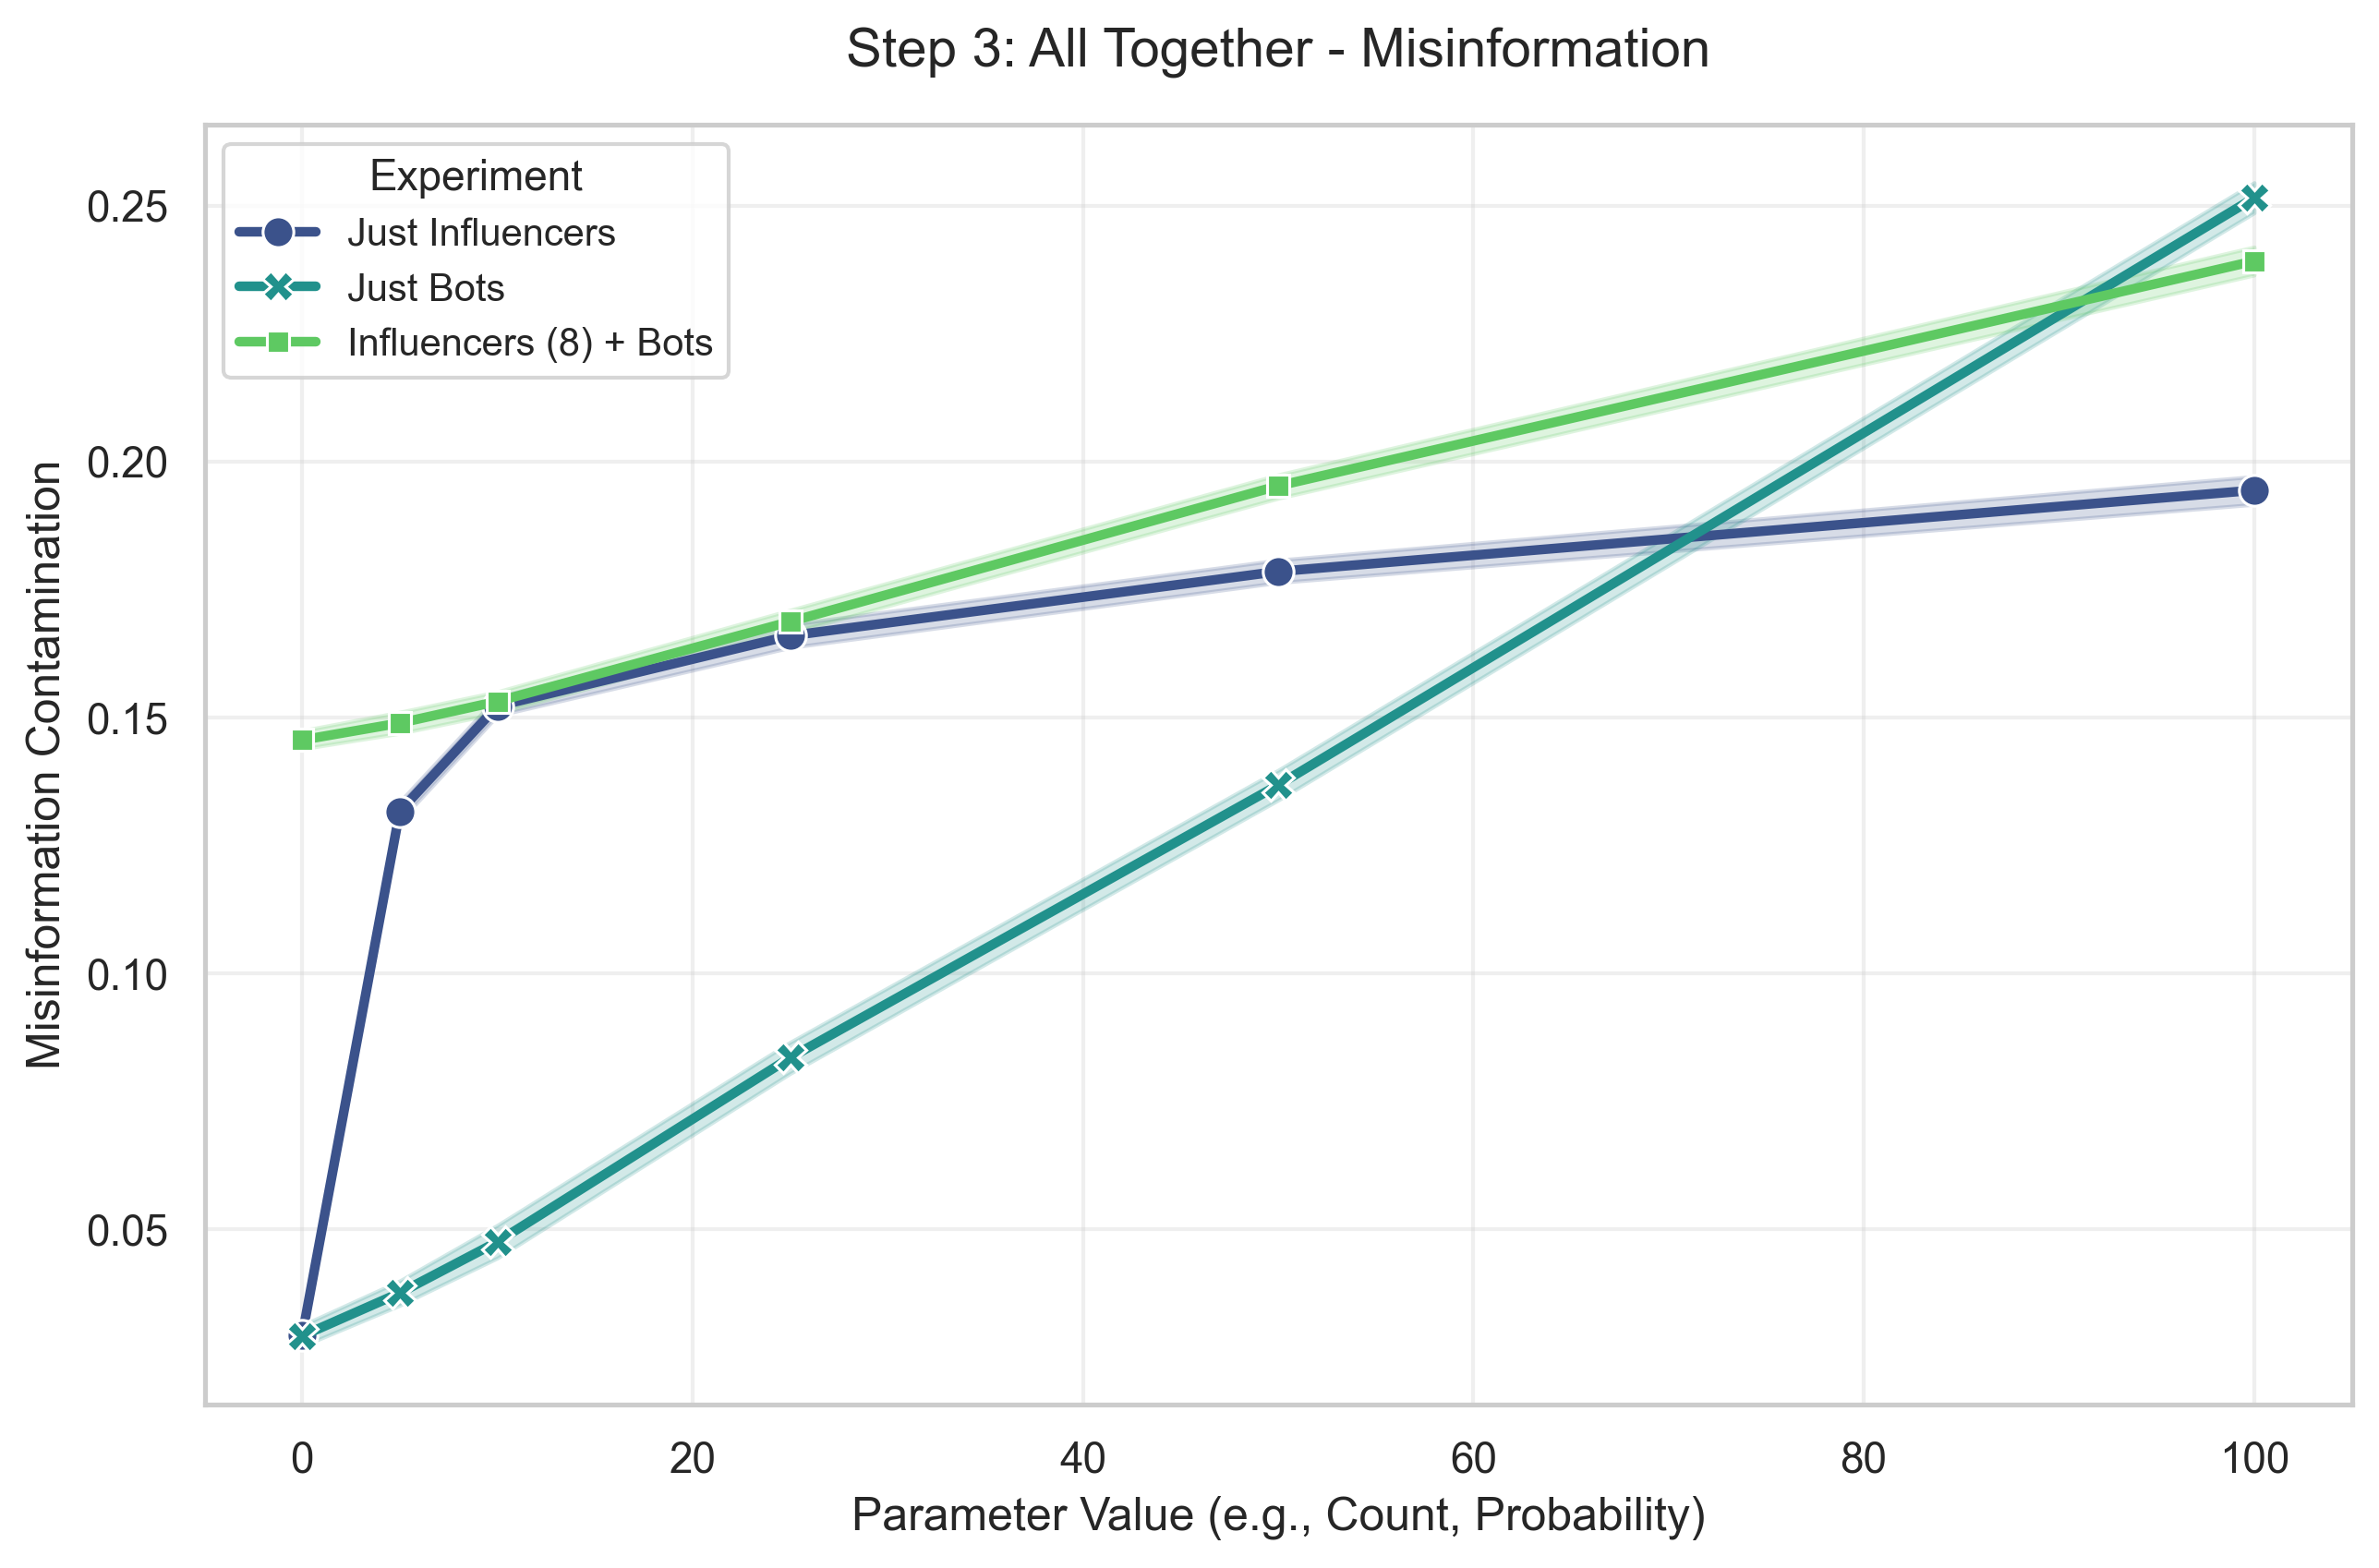
\includegraphics[width=0.8\textwidth]{figures/misinformation_step3_all.png}
\caption{Misinformation contamination patterns across agent types, showing how bots amplify spread despite filtering by high-reputation agents.}
\label{fig:misinformation_step3}
\end{figure}

Figure~\ref{fig:forwarding_step3} demonstrates the behavioral differences: influencers show lower forwarding rates due to reputation concerns, while bots forward more indiscriminately. Regular users exhibit moderate forwarding behavior, facilitating message propagation across network clusters.

\begin{figure}[H]
\centering
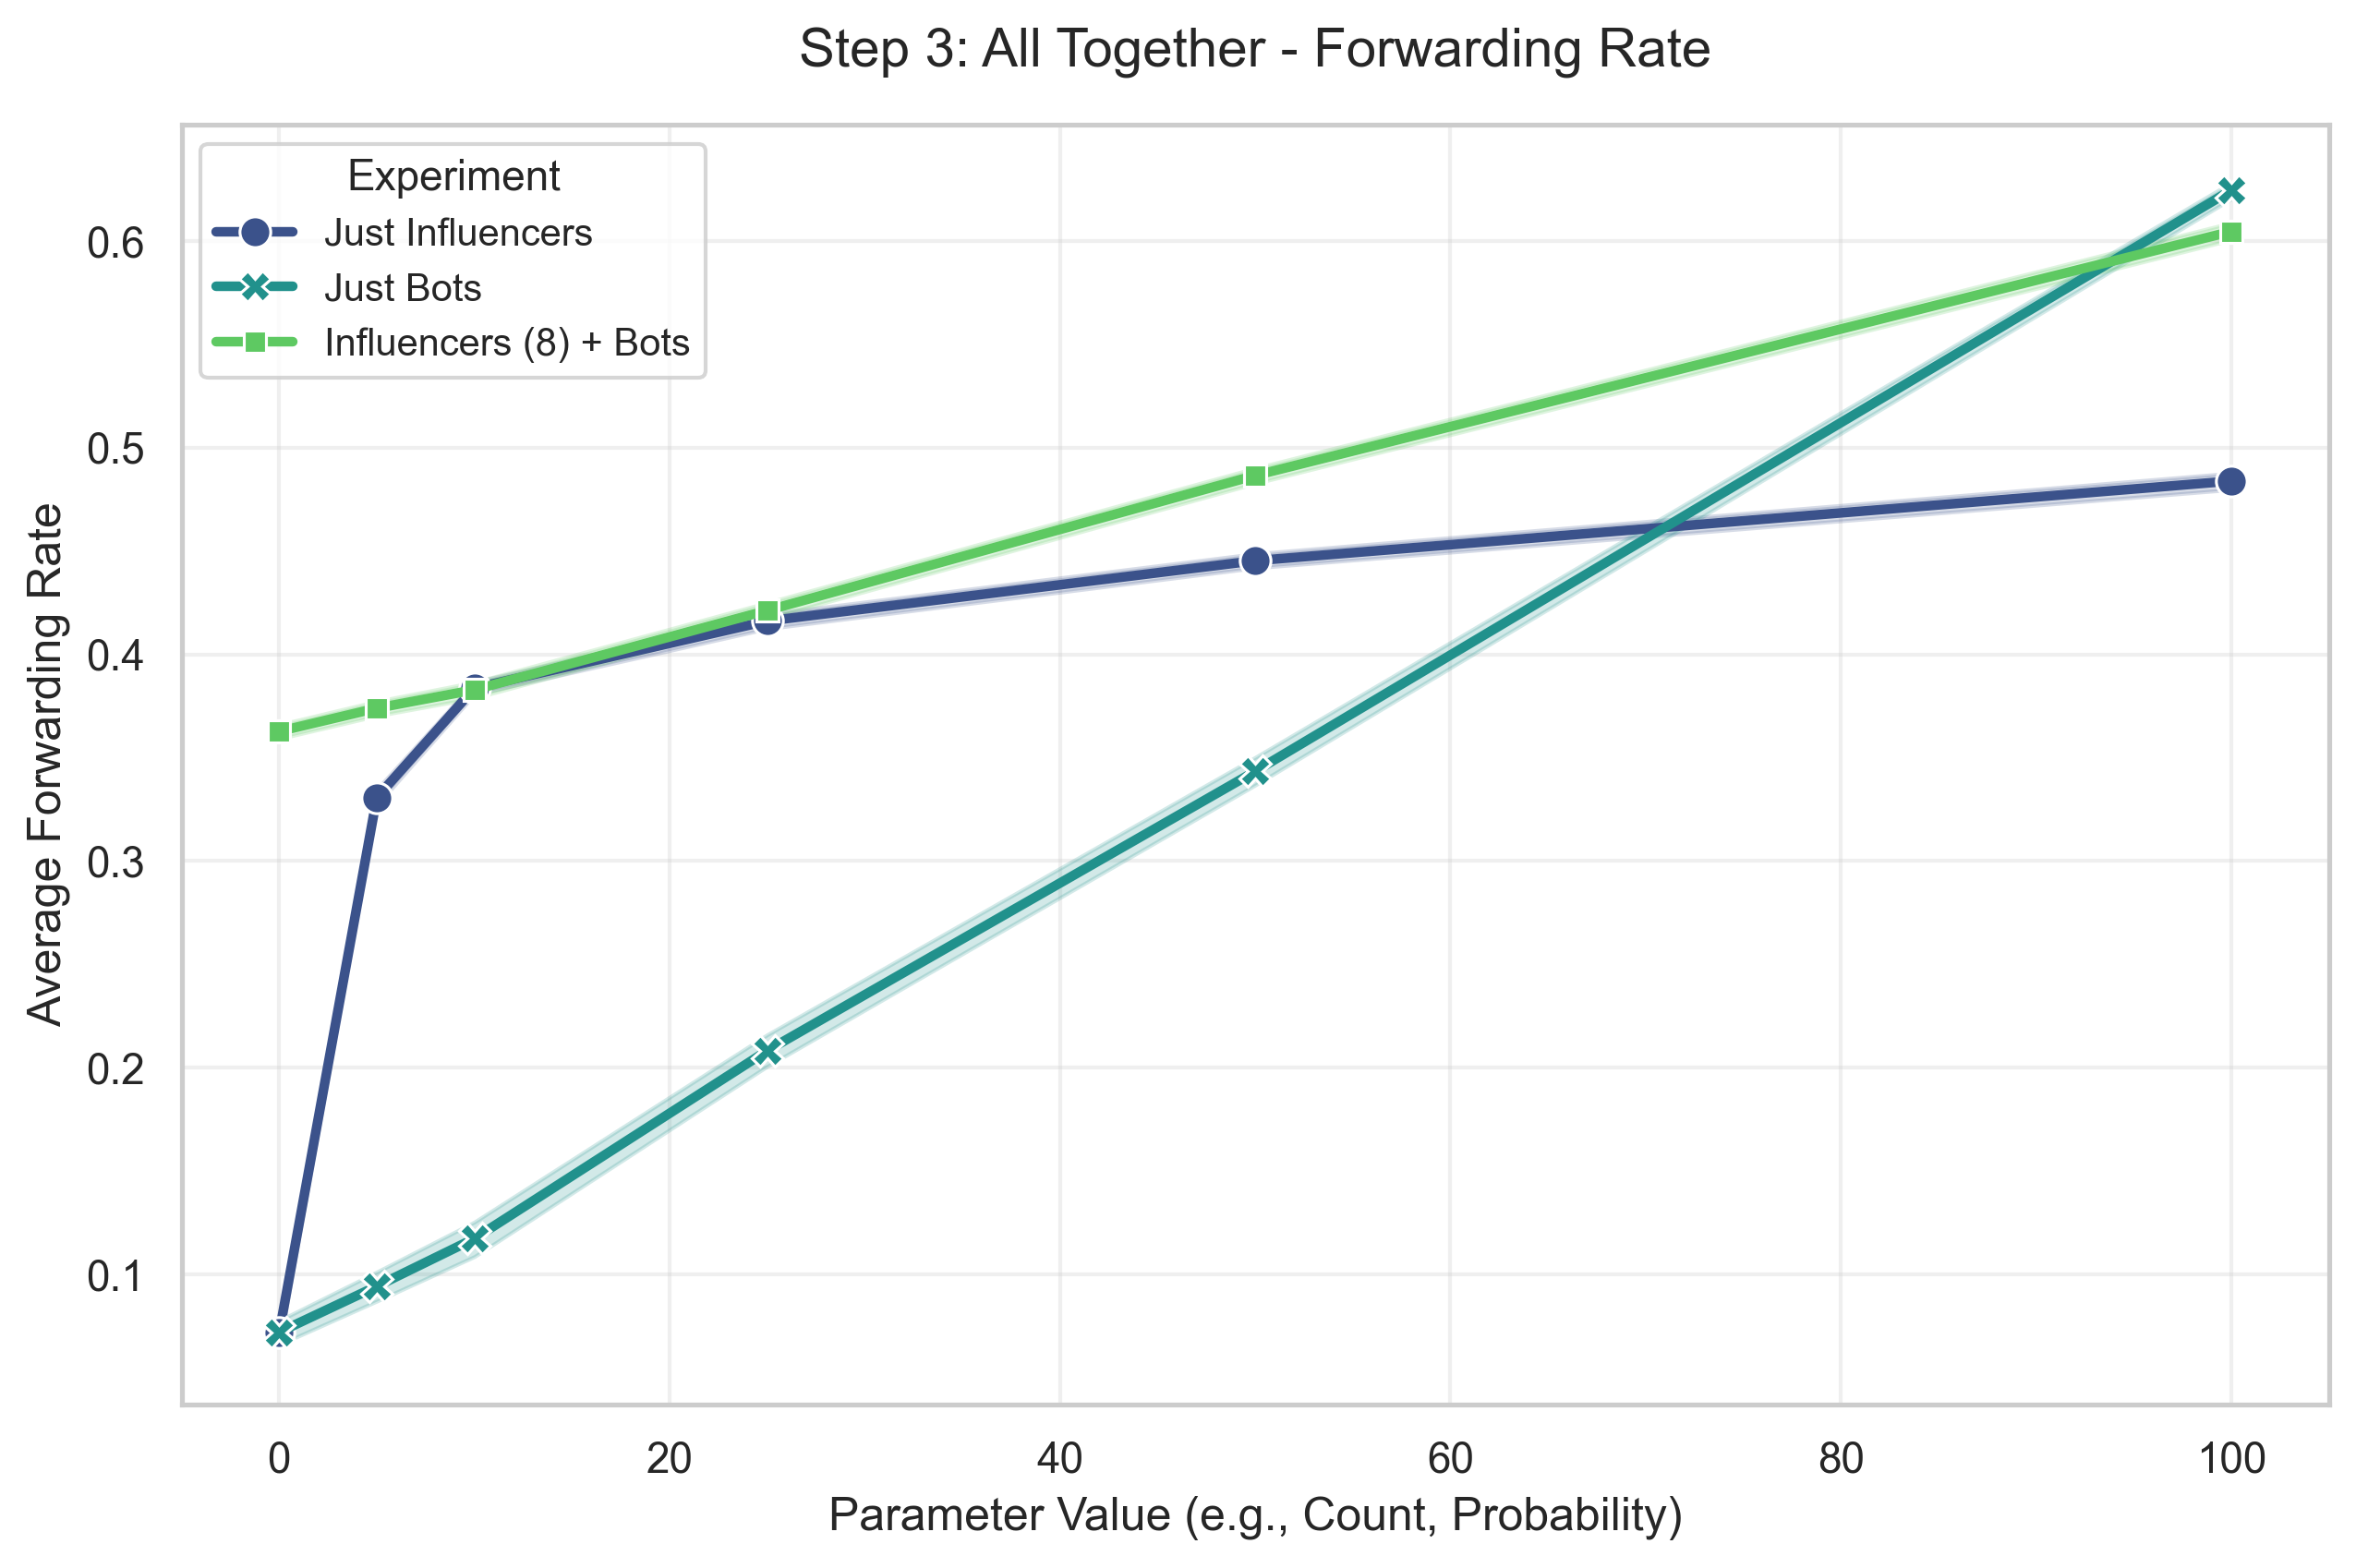
\includegraphics[width=0.8\textwidth]{figures/forwarding_step3_all.png}
\caption{Forwarding rates by agent type, illustrating how reputation sensitivity shapes forwarding decisions.}
\label{fig:forwarding_step3}
\end{figure}

\subsection{Fact-Checking Ratio and Platform Comparison}

Platforms differ significantly in their fact-checking capabilities. We abstract fact-checking as \textit{truth revelation}: after each round, the true state of the message may be revealed to agents with some probability. A higher truth-revelation probability therefore corresponds to an environment with more frequent (or more effective) fact-checking, while a lower value captures settings where verification is rare.

In our model, when truth is revealed, agents use the actual truth value $\truth$ in their utility calculation; when it is not revealed, they rely on beliefs $\widehat{\truth}$ formed from ideological proximity and sender reputation.

We compare two scenarios: (i) \textit{High fact-checking} (WhatsApp-like), where a larger fraction of messages are fact-checked and truth is observable, and (ii) \textit{Low fact-checking} (Telegram-like), where most messages lack verification and agents must rely on reputation and ideology cues.

\subsubsection{High Fact-Checking Regime (WhatsApp-like)}

When fact-checking is frequent, agents observe message truthfulness more often, which activates reputation updating more regularly. Combined with the reputation-dependent penalty $\delta(\R)$, this changes who continues to forward messages---and therefore how far messages travel (see Figures~\ref{fig:platform_reach_vs_truth_revelation_prob}--\ref{fig:platform_false_reach_count_vs_truth_revelation_prob}).

\begin{itemize}
    \item \textbf{Decreased absolute reach}: With more frequent verification, high-reputation agents become more cautious because incorrect forwarding is penalized more strongly. Since these agents typically sit in central network positions, their lower forwarding activity reduces overall reach (Figure~\ref{fig:platform_reach_vs_truth_revelation_prob}).
    
    \item \textbf{Decreased absolute false reach}: As fewer messages propagate widely, fewer agents are exposed to false messages in absolute terms (Figure~\ref{fig:platform_false_reach_count_vs_truth_revelation_prob}).
    
    \item \textbf{Increased proportional contamination}: Even as exposure falls in levels, the share of false content among messages that still circulate can rise (Figure~\ref{fig:platform_avg_misinformation_vs_truth_revelation_prob}). Intuitively, once high-reputation agents step back, diffusion is driven relatively more by low-reputation agents and bots, who face weaker penalties and are more willing to forward low-confidence content.
    
    \item \textbf{A selection channel}: The apparent paradox is therefore compositional. Stronger verification pushes the most selective (high-reputation) agents to forward less, leaving a larger role for less selective agents; this reduces false spread in absolute terms (Figure~\ref{fig:platform_false_reach_count_vs_truth_revelation_prob}), but can increase it in proportion among remaining transmissions (Figure~\ref{fig:platform_avg_misinformation_vs_truth_revelation_prob}).
\end{itemize}

\subsubsection{Low Fact-Checking Regime (Telegram-like)}

When fact-checking is rare, agents must rely primarily on reputation and ideological signals to form beliefs. This regime reveals the full force of the reputation-based mechanism:

\begin{itemize}
    \item \textbf{Higher misinformation contamination}: Without direct truth signals, agents rely more heavily on reputation and ideology, leading to higher false-forward rates. Contamination increases significantly, particularly for messages that align with agents' ideological biases (low truth-revelation probabilities in Figure~\ref{fig:platform_avg_misinformation_vs_truth_revelation_prob}).
    
    \item \textbf{Strengthened reputation premium}: The reputation mechanism becomes more powerful when verification is scarce. High-reputation agents gain a larger advantage because their reputation serves as a crucial signal for other agents, increasing reputation inequality across agent types (consistent with the mechanism in Figure~\ref{fig:reputation_step3}).
    
    \item \textbf{Ideological echo chambers}: With limited fact-checking, ideological alignment becomes a primary belief signal. Messages aligned with agents' biases are more likely to be forwarded, even when false, creating stronger echo-chamber dynamics (low truth-revelation probabilities in Figures~\ref{fig:platform_reach_vs_truth_revelation_prob} and~\ref{fig:platform_avg_misinformation_vs_truth_revelation_prob}).
\end{itemize}

\subsubsection{Comparative Impact}

The comparison highlights a key policy implication: fact-checking does not only change beliefs; it also reshapes diffusion by shifting who remains active in forwarding.

In high fact-checking environments (WhatsApp), more frequent verification activates reputation penalties more often, making high-reputation agents markedly more selective. Because these agents have outsized network influence, their withdrawal reduces overall reach and lowers false reach in absolute terms. At the same time, the messages that continue to circulate are disproportionately carried by less selective agents, which can raise the proportional contamination rate.

In low fact-checking environments (Telegram), verification is scarce and reputation becomes the main credibility cue. High-reputation agents still filter, but because the truth is revealed less often, the reputational consequences are triggered less frequently and selectivity is weaker than under high fact-checking. This creates room for low-reputation agents (especially bots) to sustain diffusion of false content, raising absolute contamination.

Overall, fact-checking and reputation-based filtering interact through an endogenous selection mechanism: stronger verification increases the effective penalty borne by high-reputation agents, reducing their forwarding activity, which lowers false exposure in levels but can concentrate misinformation among the remaining diffusion paths. Finally, the magnitude of any reduction in false-message spread---especially when measured in percentages---depends critically on the prevalence of bots (agents who share regardless of truthfulness): reducing the number of bots mechanically strengthens the decline in false reach.

\subsubsection{Platform Comparison under Varying Fact-Checking}

To make the platform comparison more transparent, we vary the probability that message truthfulness is revealed to agents after each round (the truth-revelation probability), spanning Telegram-like (low fact-checking) to WhatsApp-like (high fact-checking). We report three complementary reach measures: overall reach, false reach as a share of the network, and false reach in absolute counts. Together, these figures highlight the selection channel discussed above: total exposure can fall while proportional contamination rises.

\begin{figure}[H]
\centering
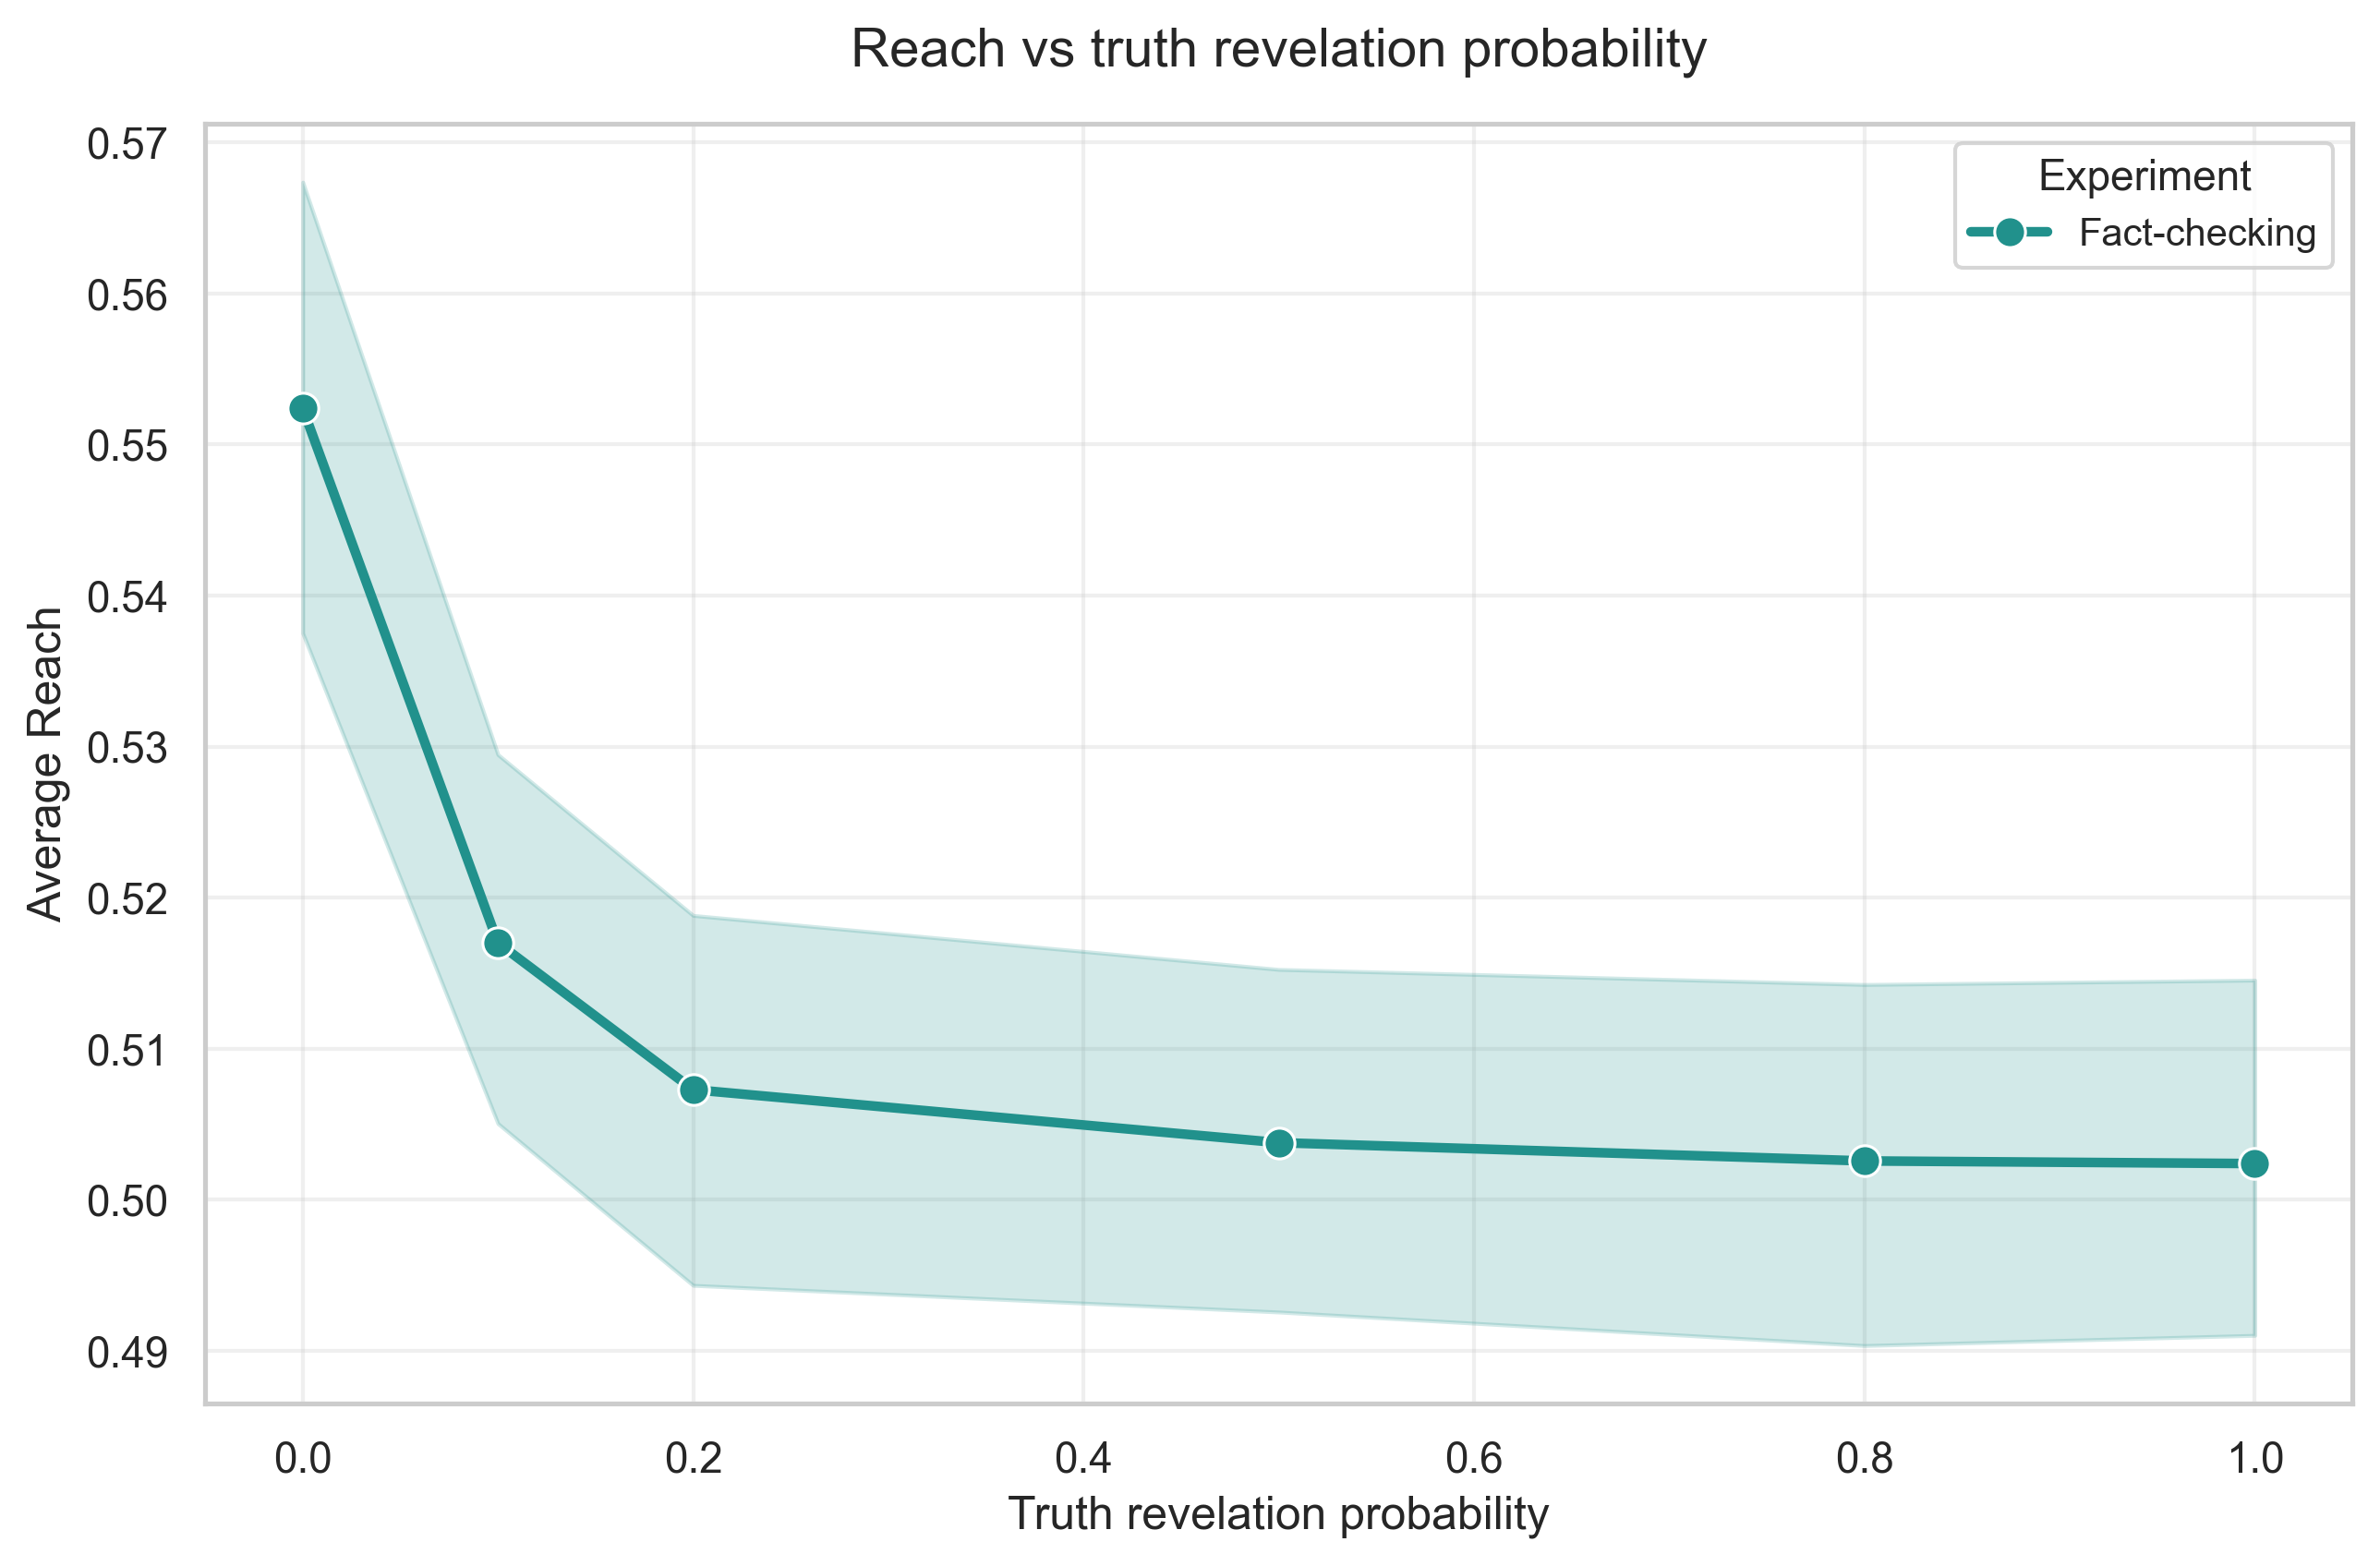
\includegraphics[width=0.9\textwidth]{figures/platform_reach_vs_truth_revelation_prob.png}
\caption{Overall message reach as the truth-revelation probability varies (low values are Telegram-like; high values are WhatsApp-like).}
\label{fig:platform_reach_vs_truth_revelation_prob}
\end{figure}

\begin{figure}[H]
    \centering
    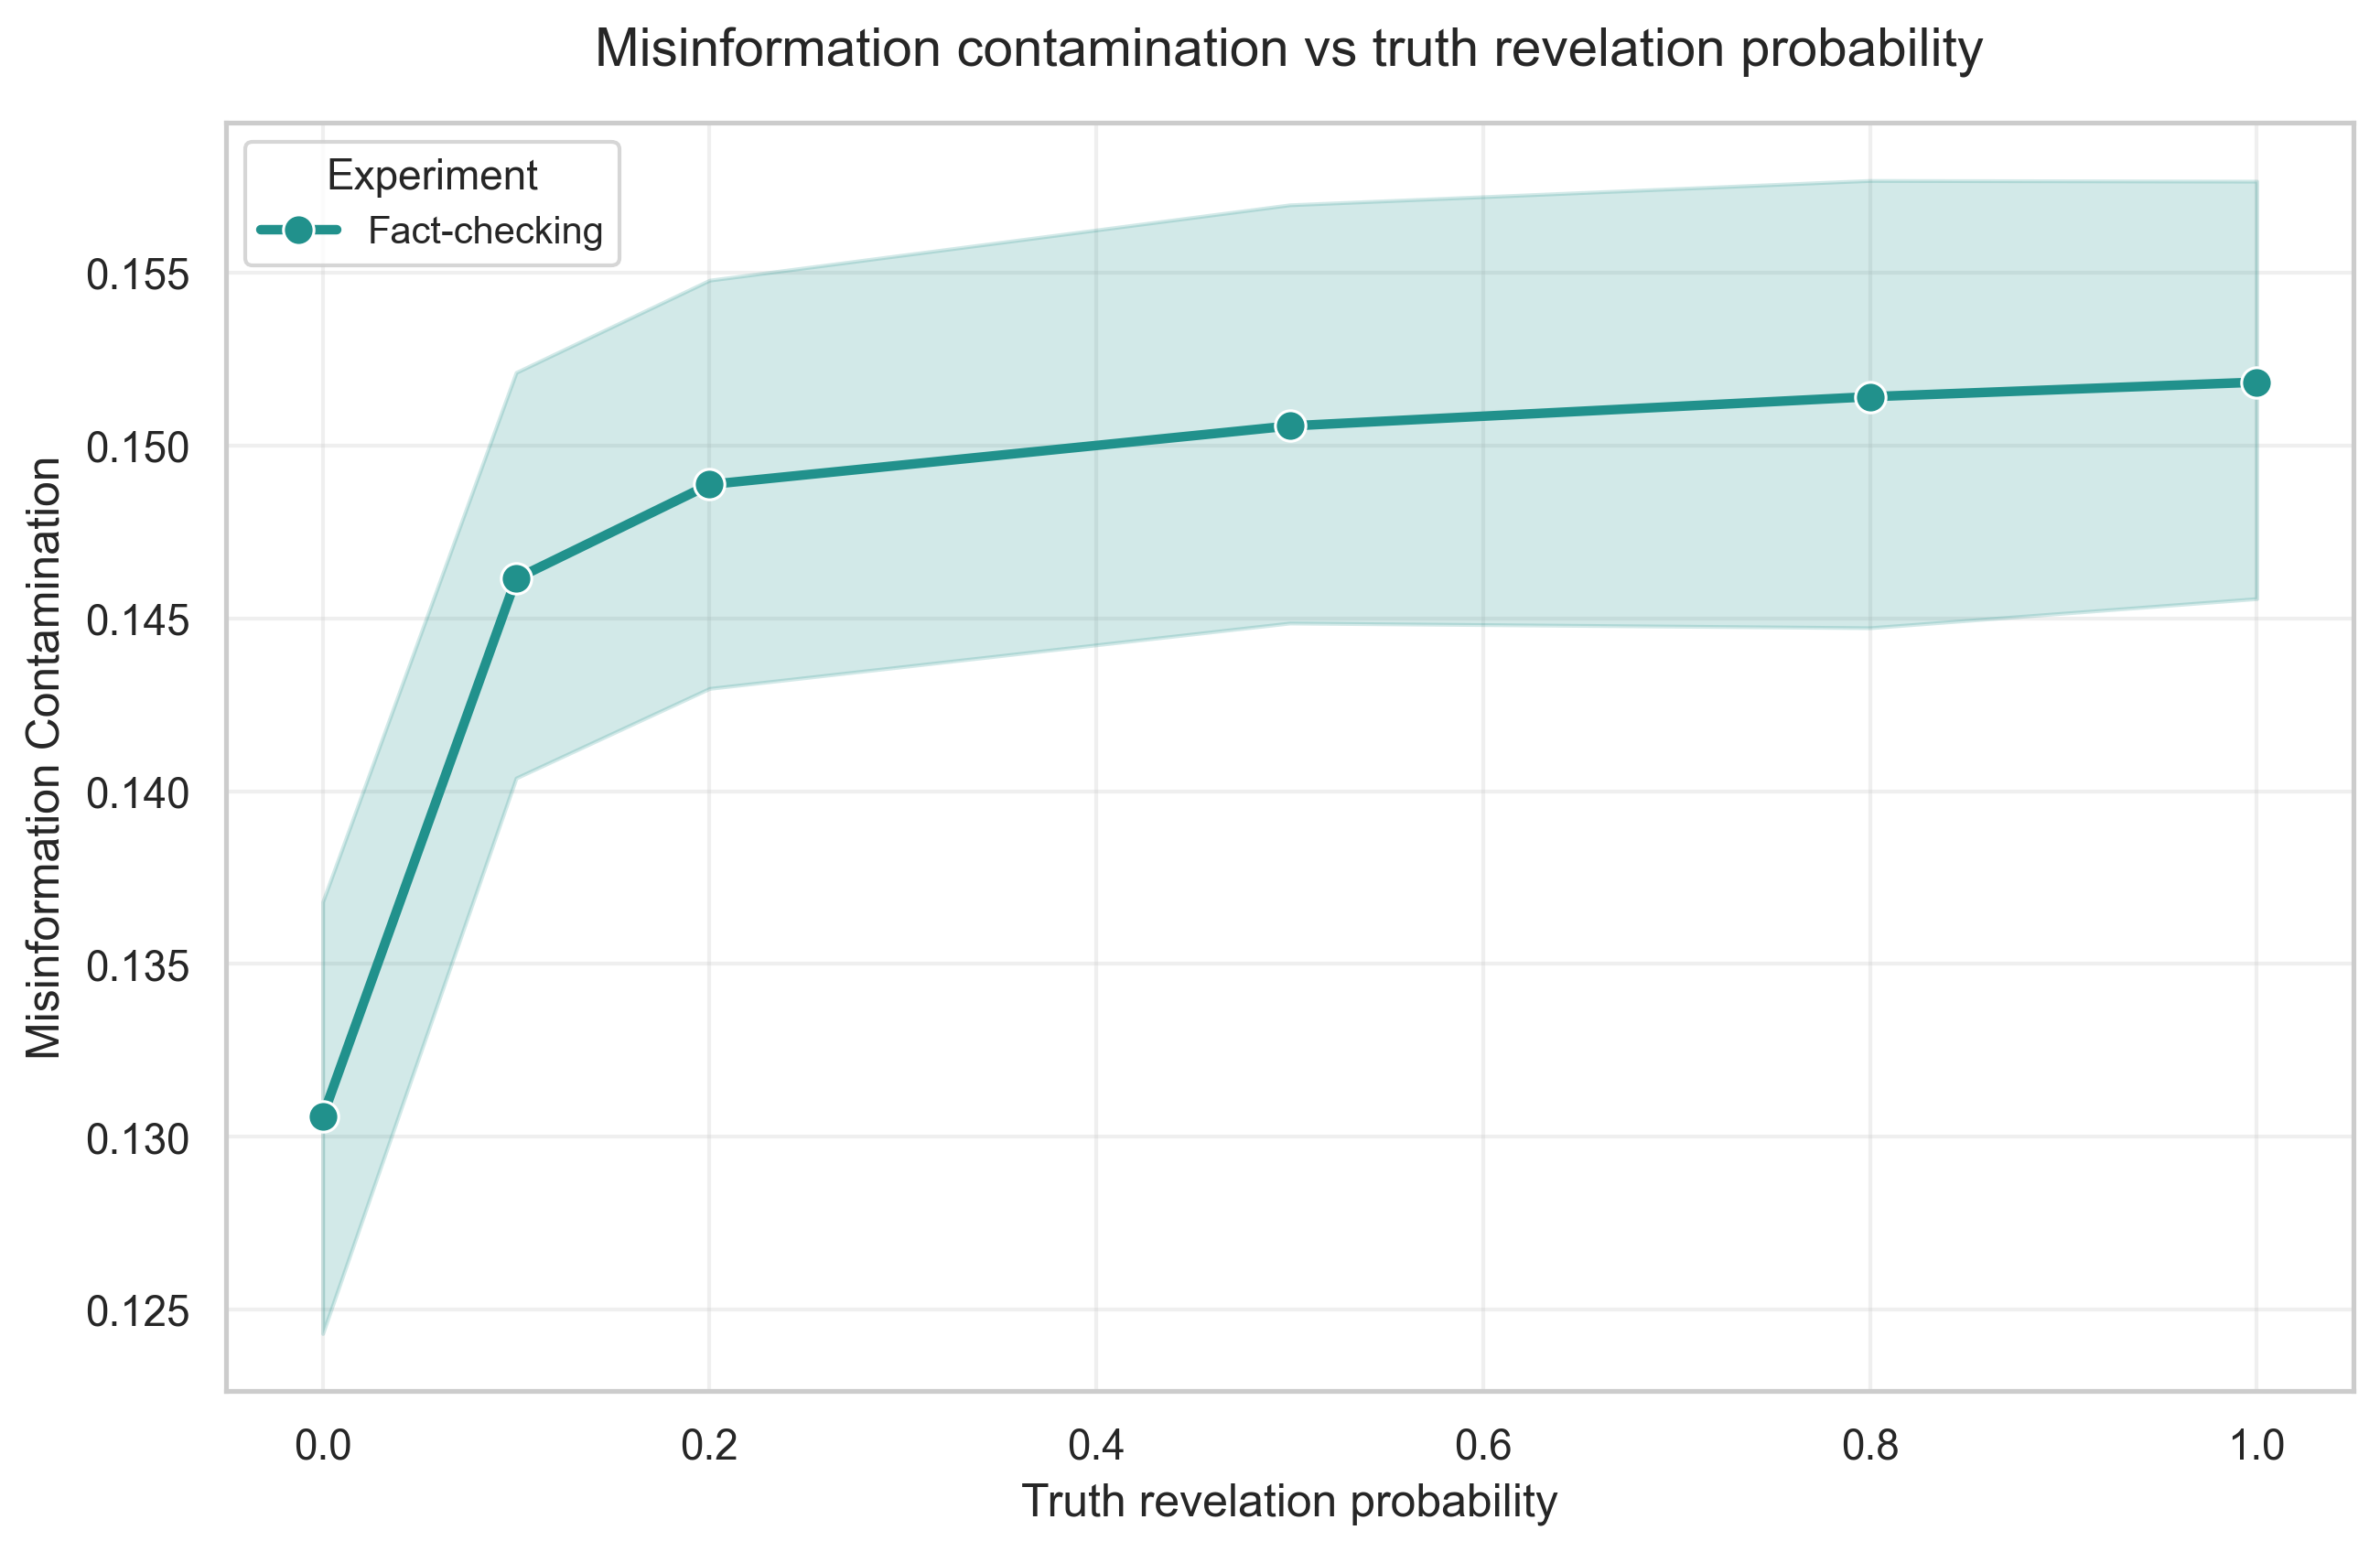
\includegraphics[width=0.9\textwidth]{figures/platform_avg_misinformation_vs_truth_revelation_prob.png}
    \caption{Misinformation contamination (proportion) as the truth-revelation probability varies.}
    \label{fig:platform_avg_misinformation_vs_truth_revelation_prob}
\end{figure}

\begin{figure}[H]
\centering
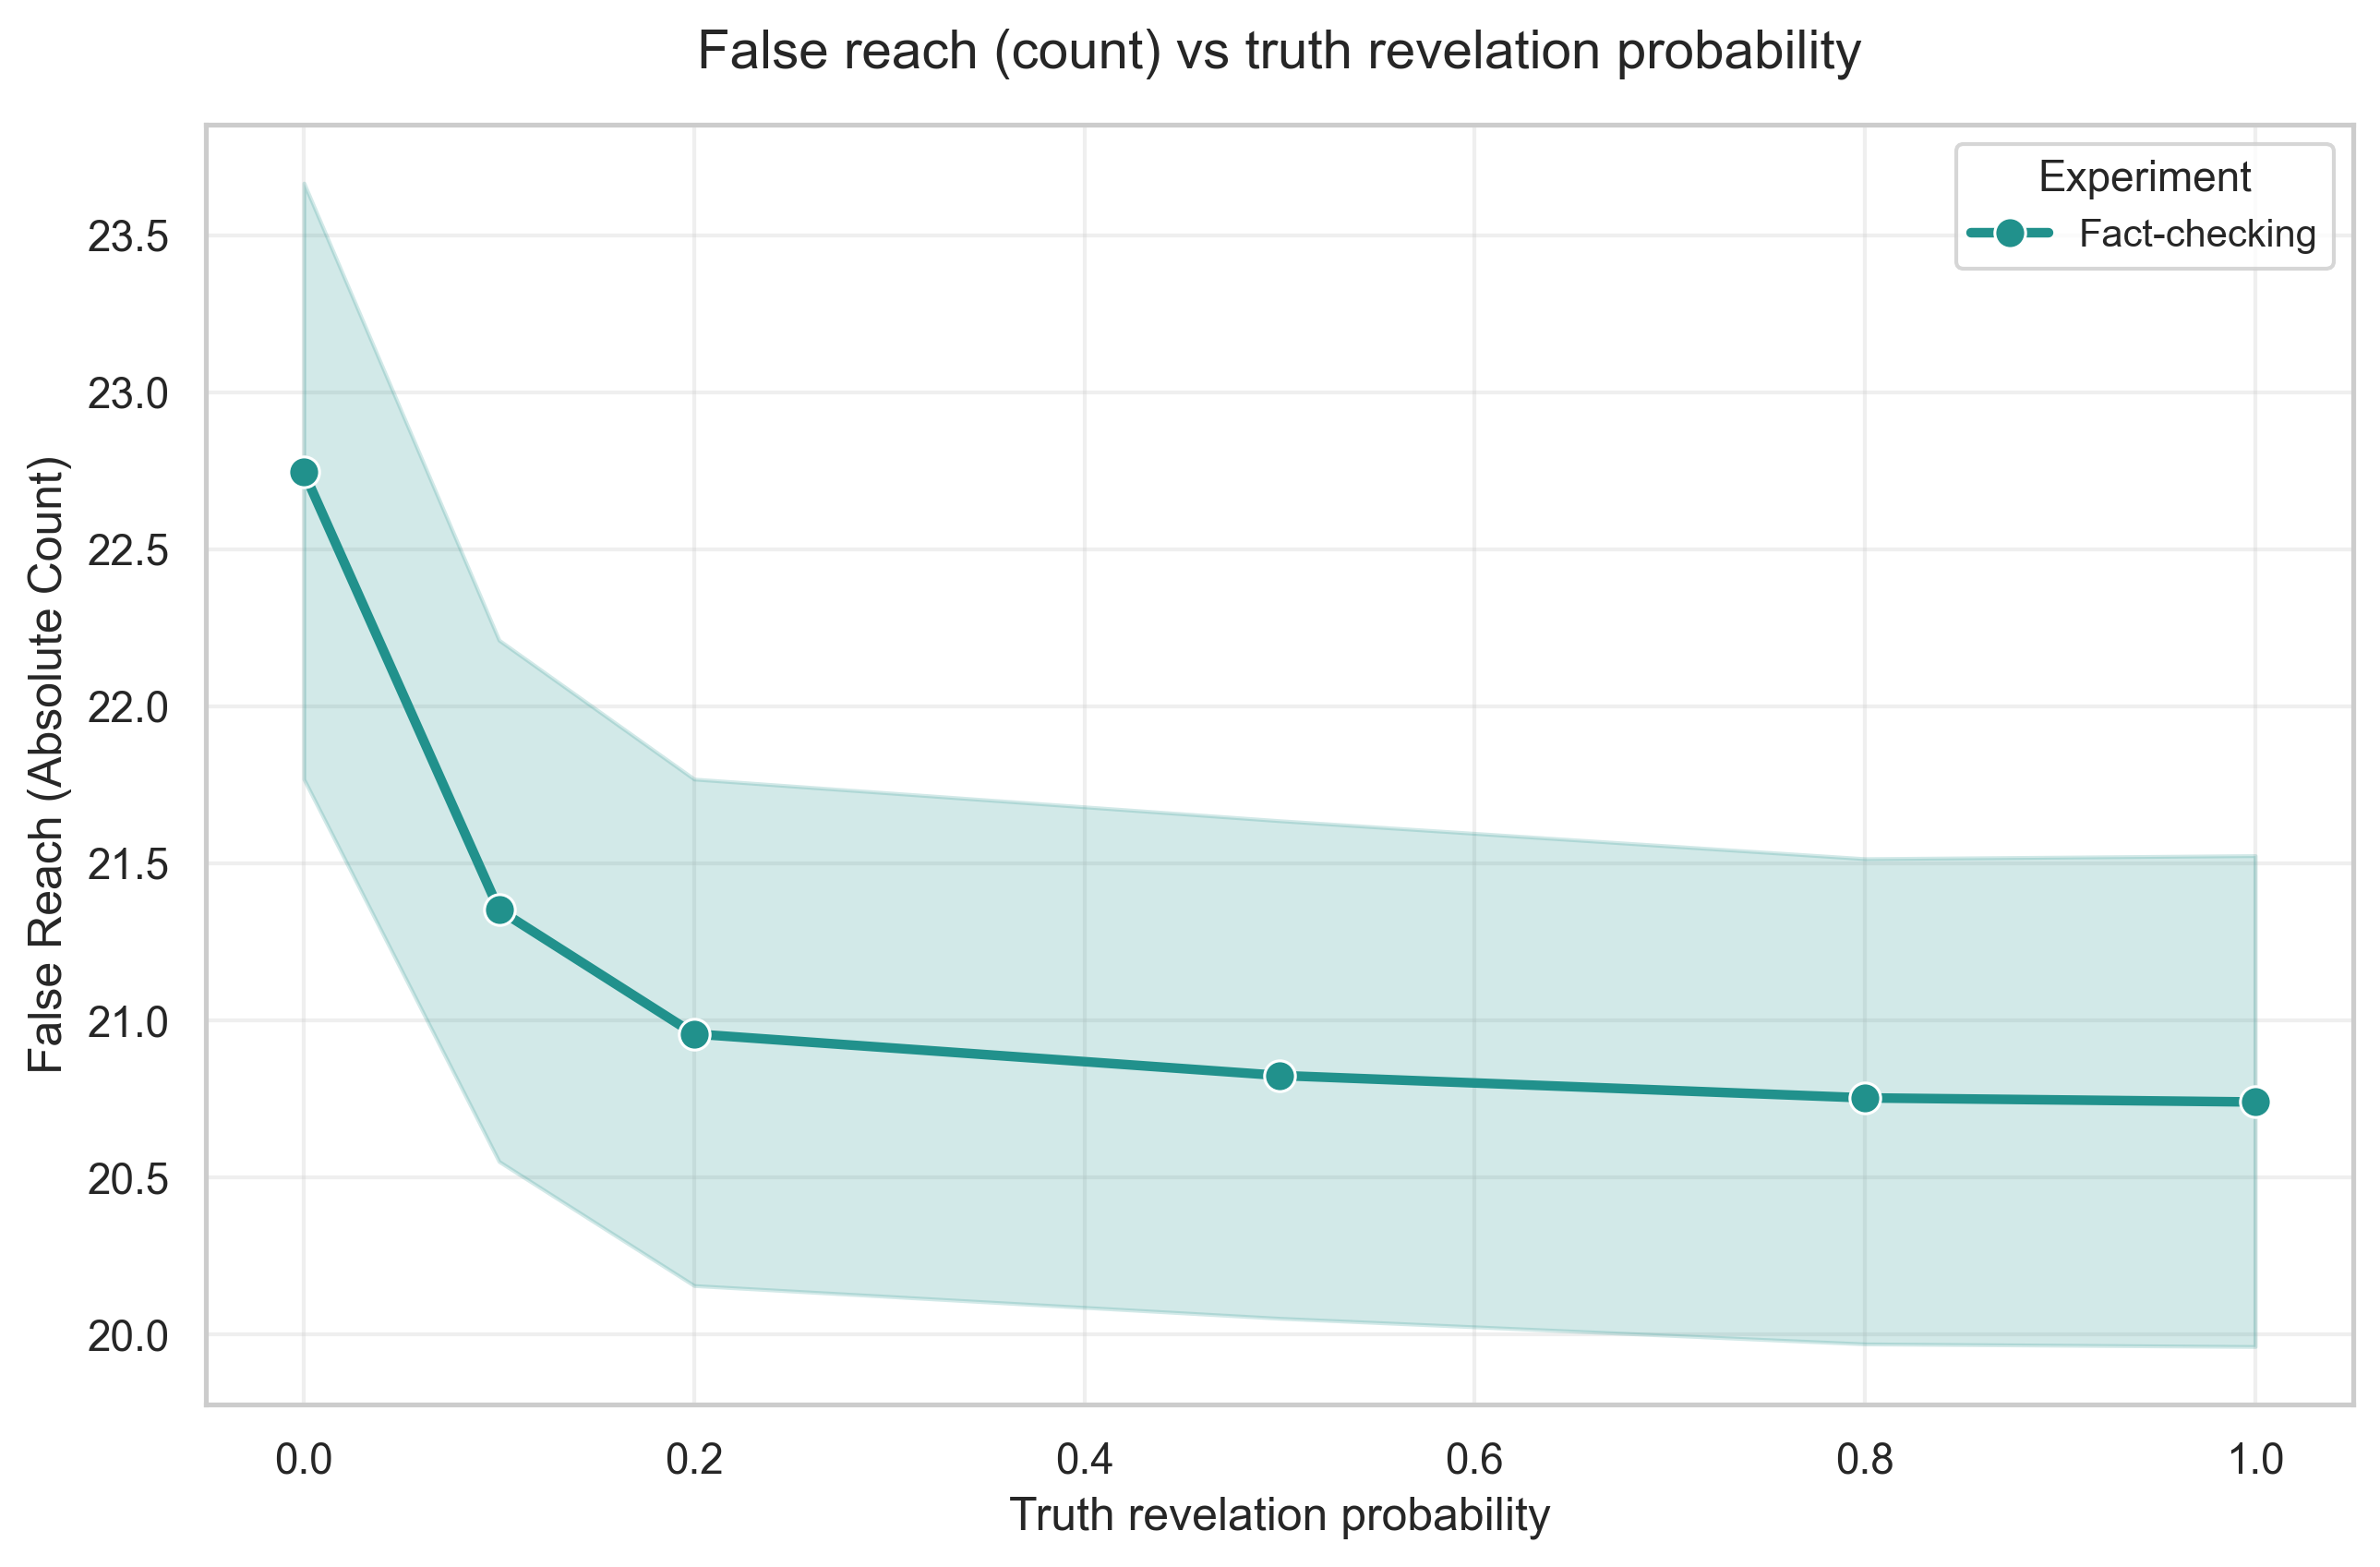
\includegraphics[width=0.9\textwidth]{figures/platform_false_reach_count_vs_truth_revelation_prob.png}
\caption{False reach (absolute number of agents exposed to false messages) as the truth-revelation probability varies.}
\label{fig:platform_false_reach_count_vs_truth_revelation_prob}
\end{figure}

\subsubsection{Bots and False-Message Spread in Telegram-like Environments}

Finally, focusing on the Telegram-like setting, we vary the number of bots and examine how false-message spread changes. Because bots forward largely irrespective of truthfulness, reductions in bots are a key driver of reductions in false spread---including when measured in percentages.

\begin{figure}[H]
\centering
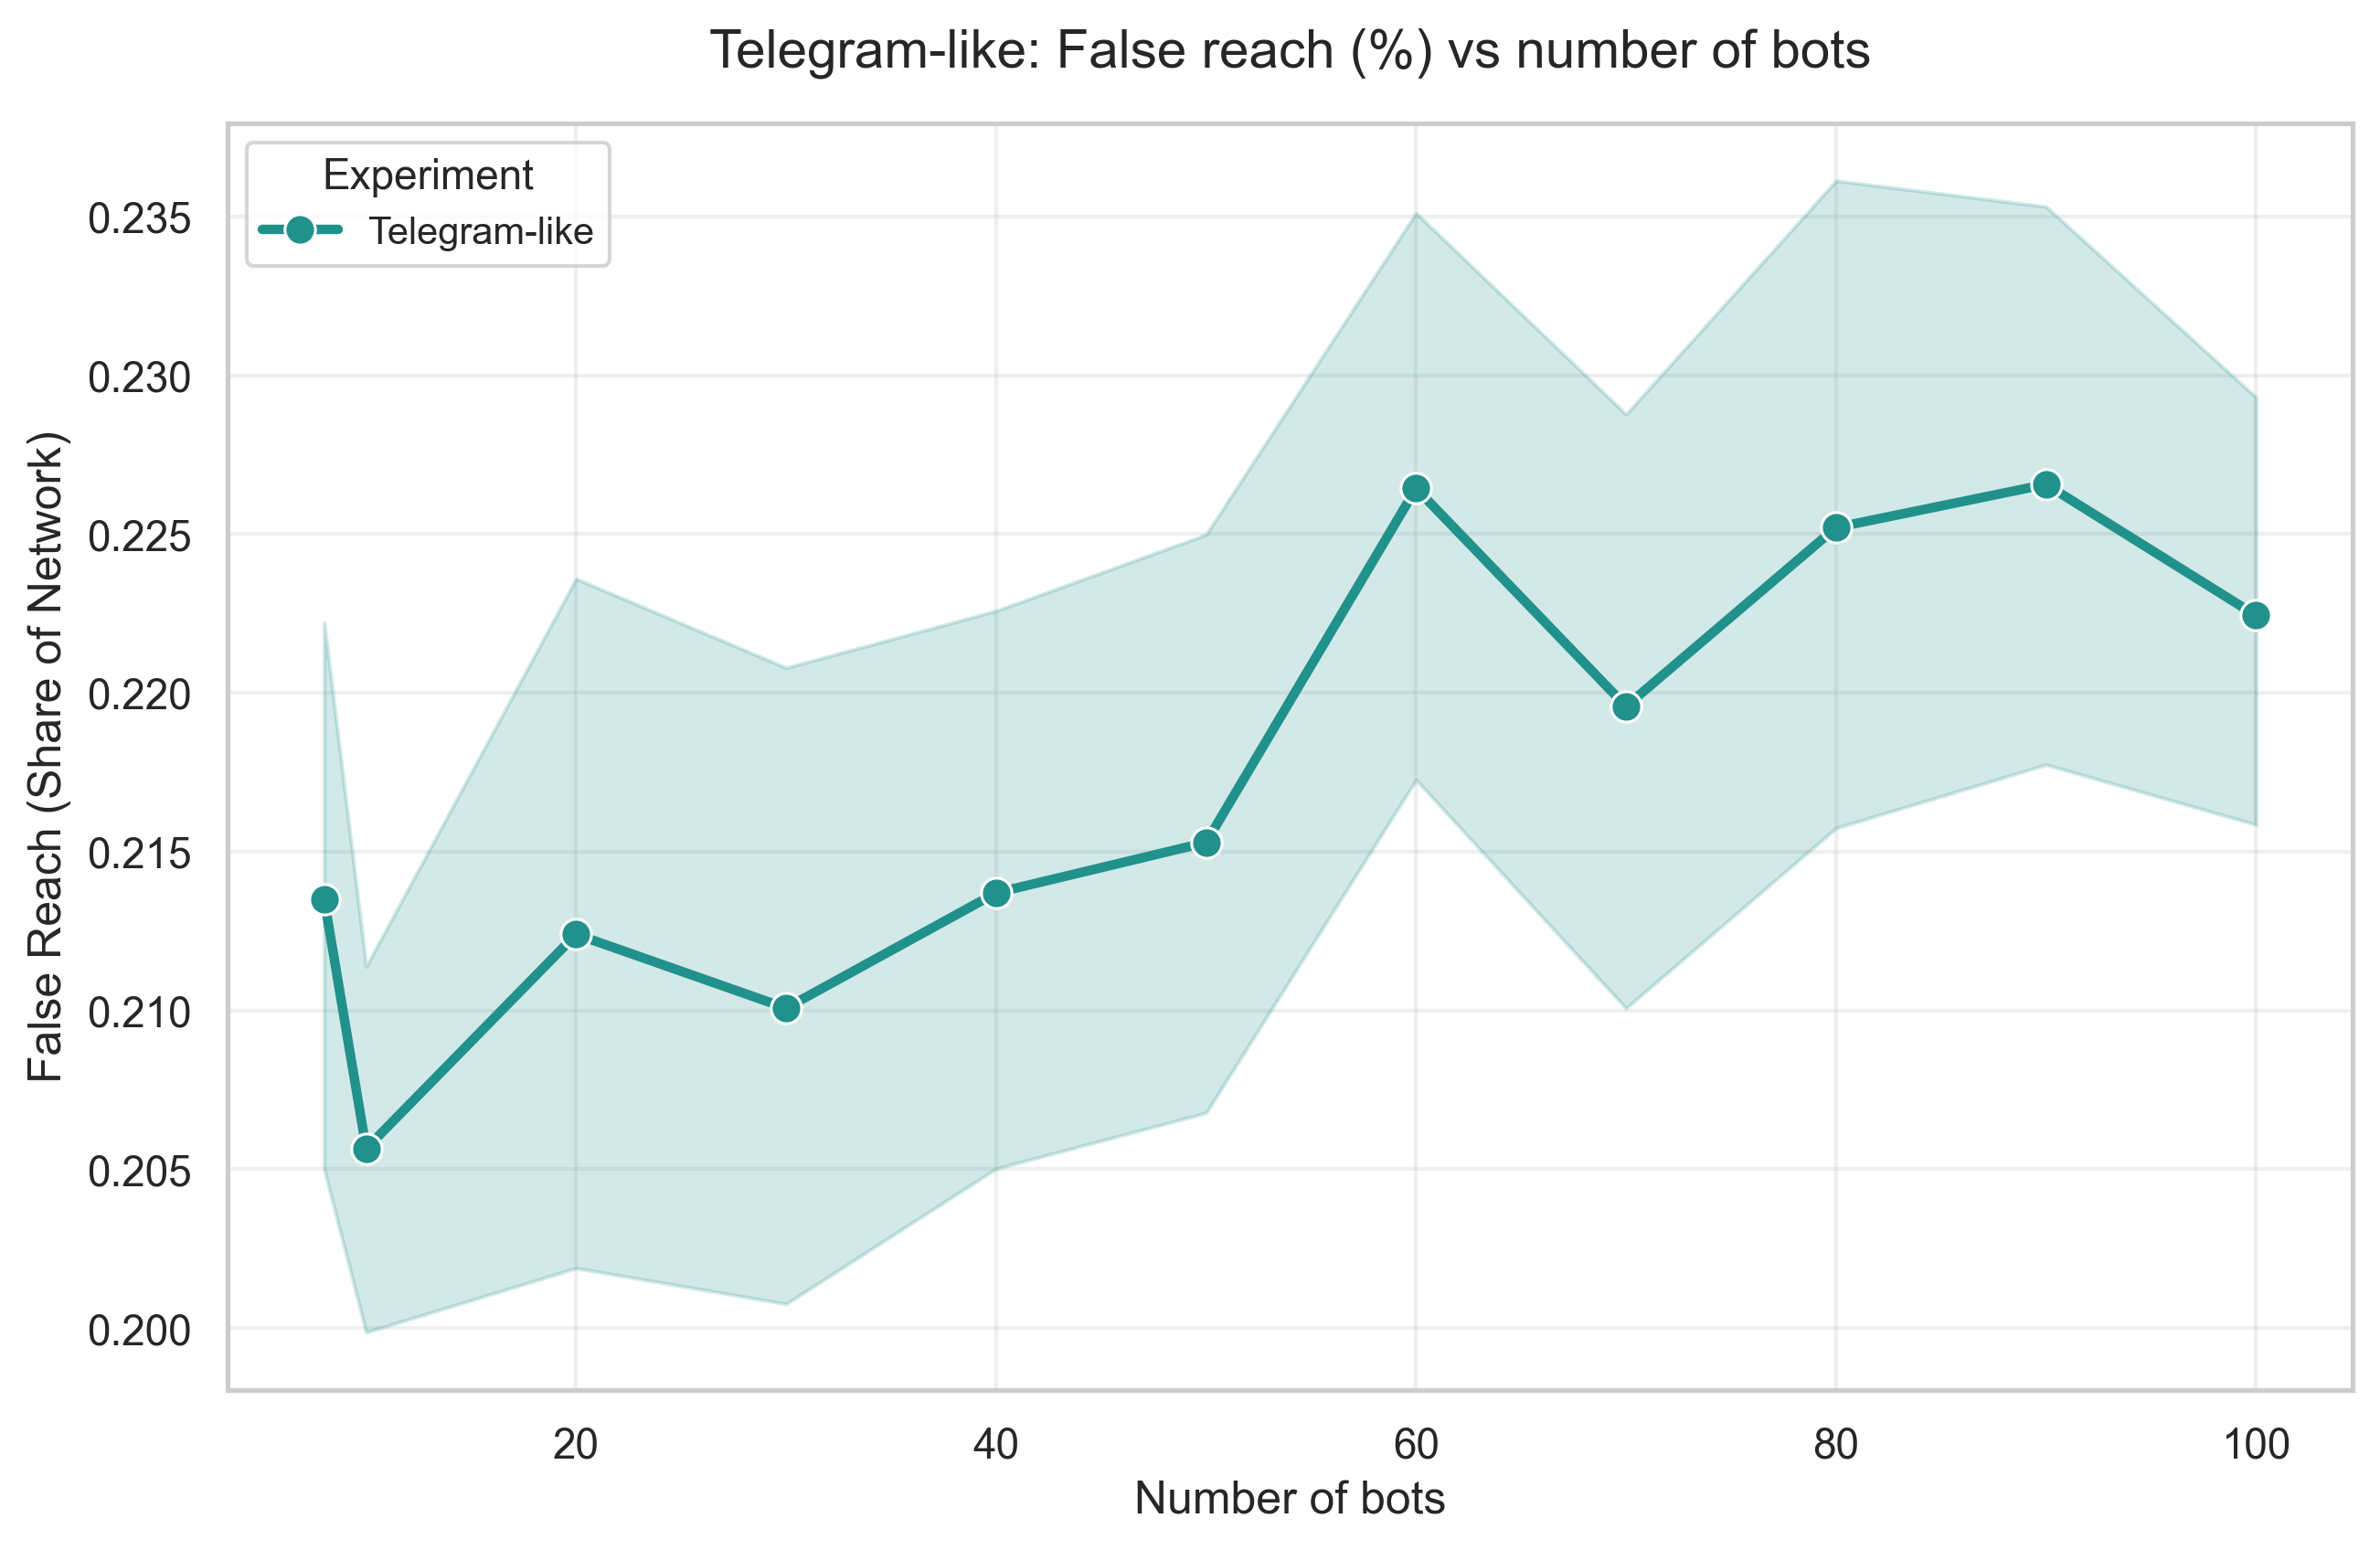
\includegraphics[width=0.9\textwidth]{figures/telegram_false_spread_vs_bots.png}
\caption{Telegram-like environment: false-message spread (percentage) as the number of bots varies.}
\label{fig:telegram_false_spread_vs_bots}
\end{figure}

\begin{figure}[H]
\centering
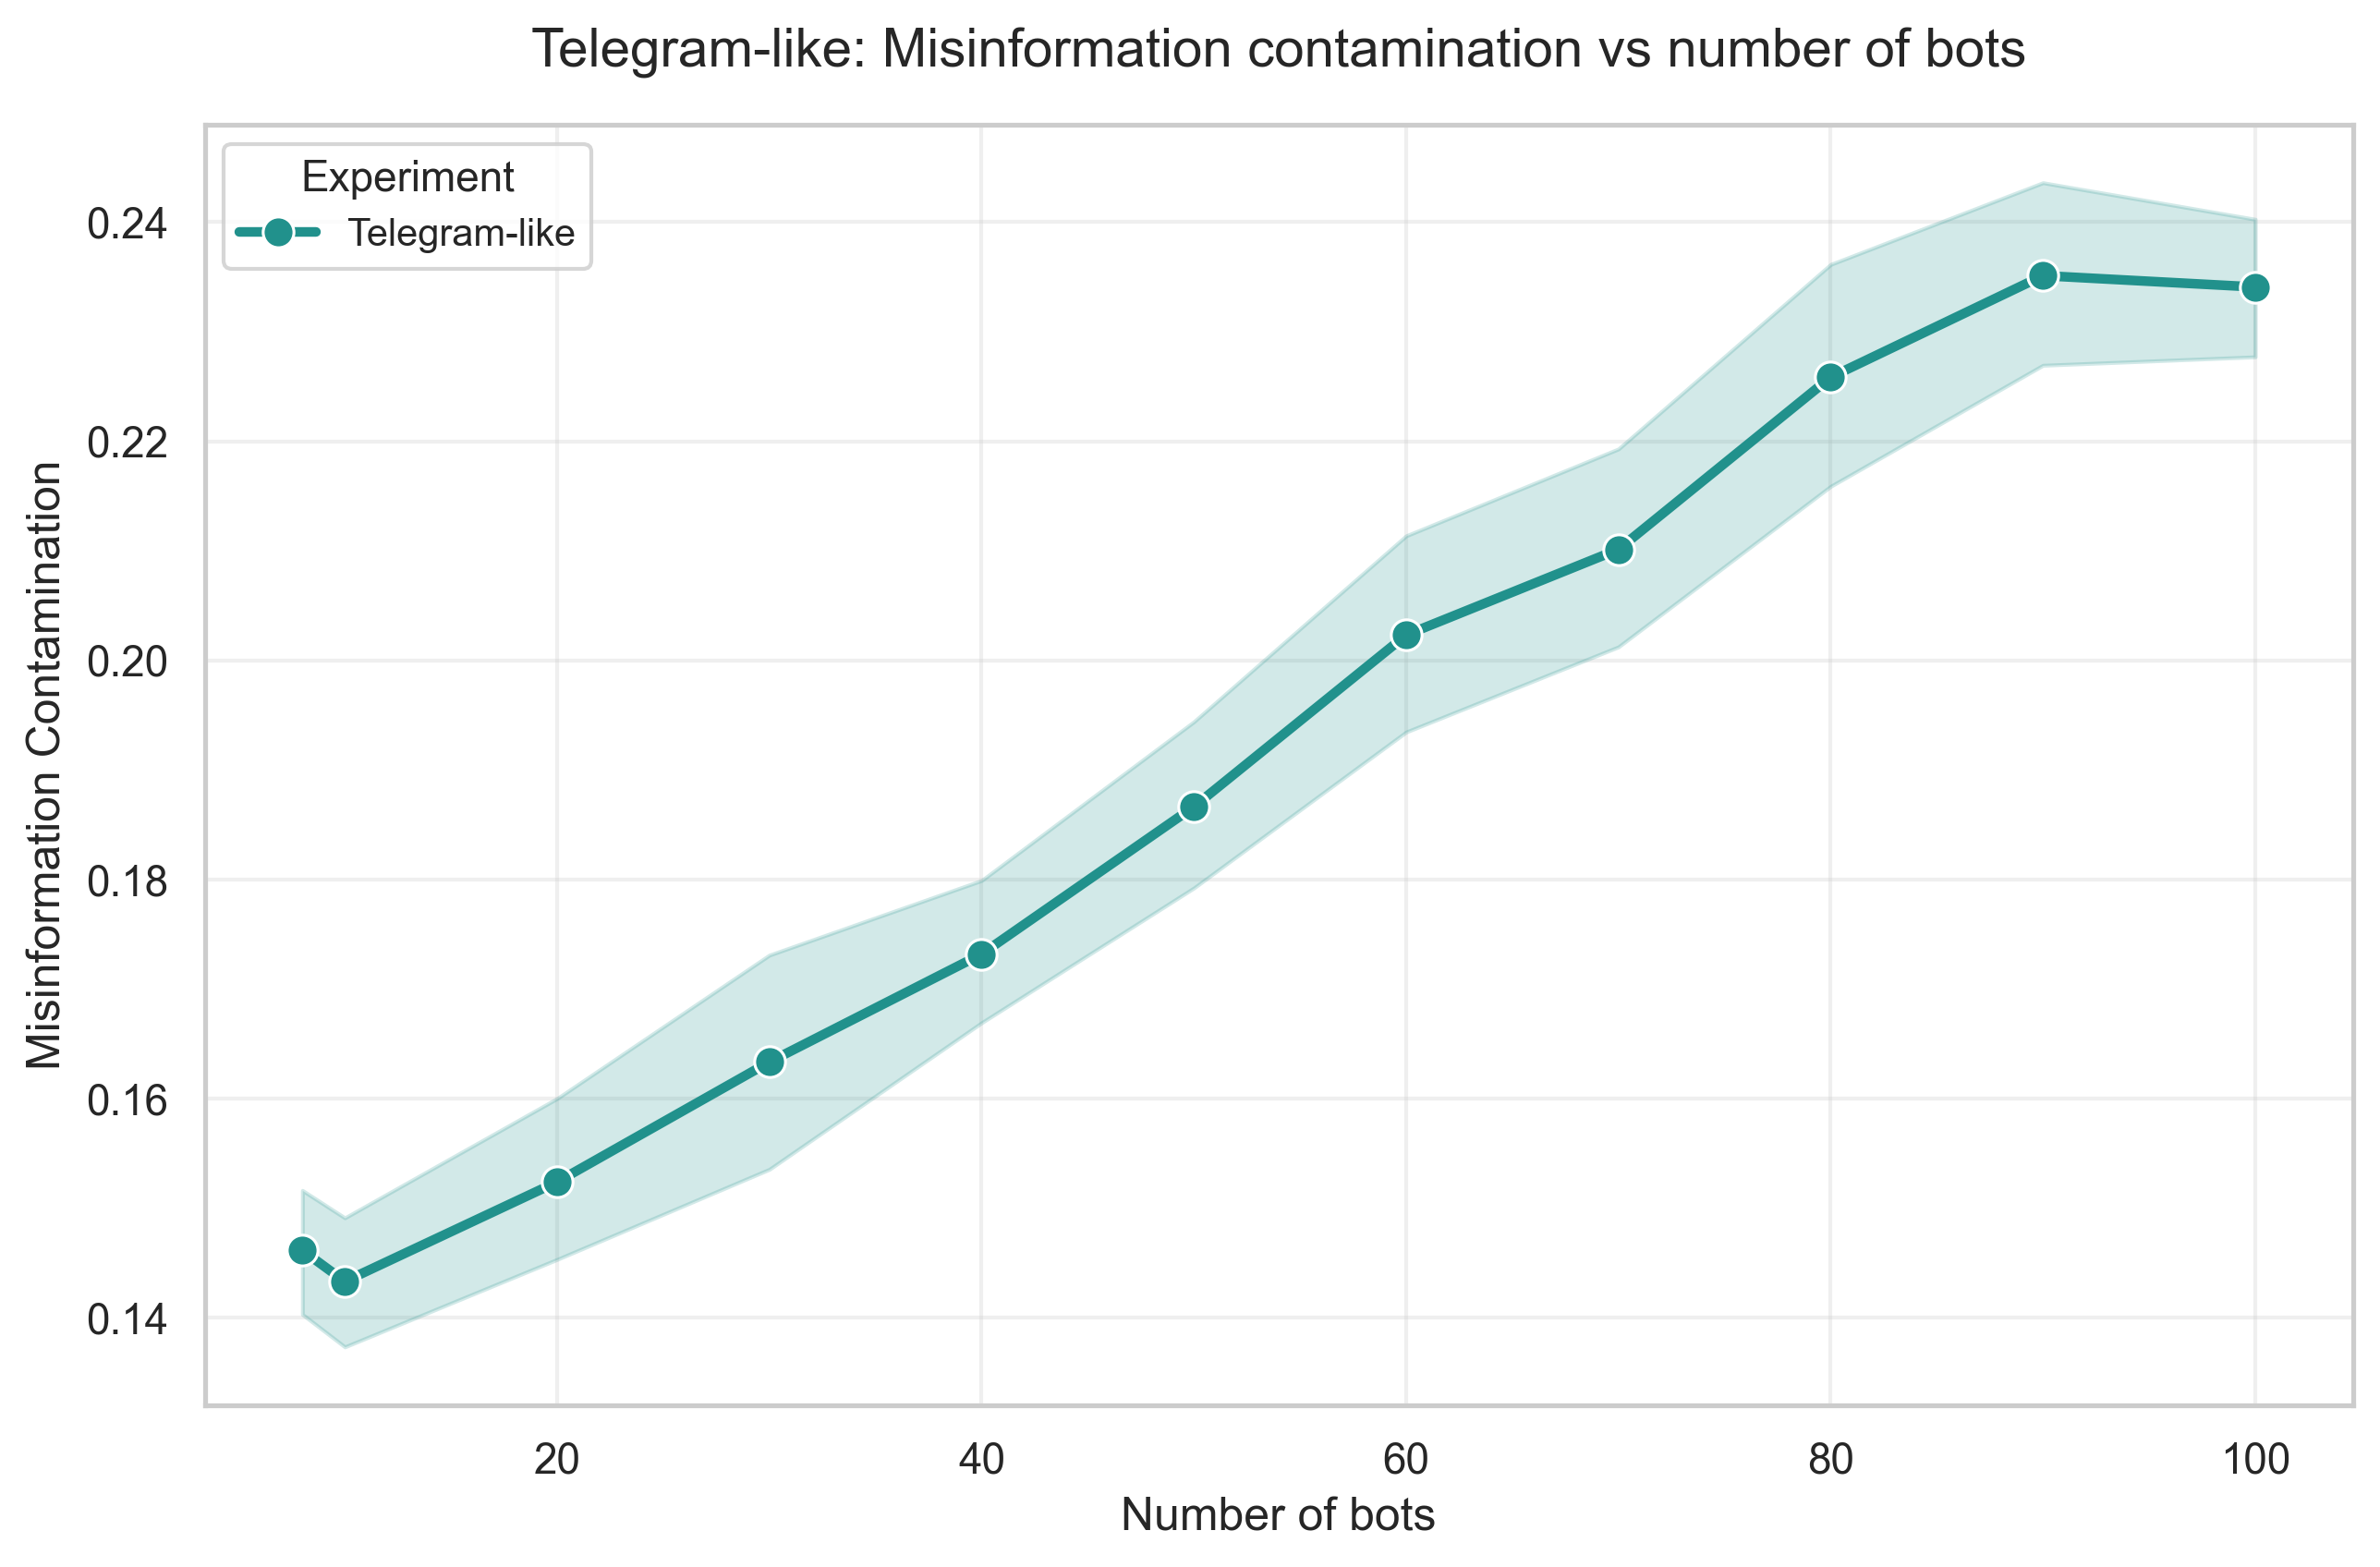
\includegraphics[width=0.9\textwidth]{figures/telegram_avg_misinformation_vs_bots.png}
\caption{Telegram-like environment: misinformation contamination (proportion) as the number of bots varies.}
\label{fig:telegram_avg_misinformation_vs_bots}
\end{figure}
